\documentclass[a4paper, 12pt, garamond]{book}
\usepackage{cours-preambule}
\usepackage{tocloft}
\usepackage{fancybox}

\renewcommand{\mtcSfont}{\Large}
\setlength{\mtcindent}{5pt}
\mtcsetoffset{minitoc}{-5pt}
\addtolength{\cftsecnumwidth}{10pt}
\setcounter{minitocdepth}{1}

\def\lspace{25}

\dominitoc
\faketableofcontents

% \toggletrue{student}
% \toggletrue{corrige}
% \renewcommand{\mycol}{black}
% \renewcommand{\mycol}{gray}

\makeatletter
\renewcommand{\@chapapp}{MPSI3 -- 12 avril 2024 -- Devoir surveillé}
\makeatother

\setlist[blocQR,1]{leftmargin=10pt, label=\sqenumi}
\counterwithin*{equation}{section}

\begin{document}
\setcounter{chapter}{8}

% \settype{enon}
% \settype{solu_prof}
% \settype{solu_stud}

\chapter{\cswitch{Correction du DS}{Thermodynamique}}
\label{ch:ds09}

\enonce{
\begin{center}
	\Large\bfseries
	Tout moyen de communication est interdit
	\smallbreak
	Les téléphones portables doivent être éteints et rangés dans les sacs
	\smallbreak
	\xul{Les calculatrices sont \textit{autorisées}}
\end{center}
\begin{tcn}[cnt, bld](ror)<itc>""{Au programme}
	\large
	Toute la thermodynamique de MPSI.
\end{tcn}

{
\vfill
\let\item\olditem
\minitoc
\vfill
}

Les différentes questions peuvent être traitées dans l'ordre désiré.
\textbf{Cependant}, vous indiquerez le numéro correct de chaque question. Vous
prendrez soin d'indiquer sur votre copie si vous reprenez une question d'un
exercice plus loin dans la copie, sous peine qu'elle ne soit ni vue ni
corrigée.
\bigbreak
Vous porterez une attention particulière à la \textbf{qualité de rédaction}.
Vous énoncerez clairement les hypothèses, les lois et théorèmes utilisés. Les
relations mathématiques doivent être reliées par des connecteurs logiques.
\bigbreak
Vous prendre soin de la \textbf{présentation} de votre copie, notamment au
niveau de l'écriture, de l'orthographe, des encadrements, de la marge et du
cadre laissé pour la note et le commentaire. Vous \textbf{encadrerez les
	expressions littérales}, sans faire apparaître les calculs. Vous ferez
apparaître cependant le détail des grandeurs avec leurs unités. Vous
\textbf{soulignerez les applications numériques}.
\bigbreak
Ainsi, l'étudiant-e s'expose aux malus suivants concernant la forme et le
fond~:
\begin{tcn}*(prop)"bomb"{Malus}
	\begin{minipage}[t]{0.50\linewidth}
		\begin{itemize}
			\item A~: application numérique mal faite~;
			\item N~: numéro de copie manquant~;
			\item P~: prénom manquant~;
			\item E~: manque d'encadrement des réponses~;
			\item M~: marge non laissée ou trop grande~;
			\item V~: confusion ou oubli de vecteurs~;
		\end{itemize}
	\end{minipage}
	\begin{minipage}[t]{0.50\linewidth}
		\begin{itemize}
			\item Q~: question mal ou non indiquée~;
			\item C~: copie grand carreaux~;
			\item U~: mauvaise unité (flagrante)~;
			\item H~: homogénéité non respectée~;
			\item S~: chiffres significatifs non cohérents~;
			\item $\f$~: loi physique fondamentale brisée.
		\end{itemize}
	\end{minipage}
\end{tcn}

% \begin{tcb}(impo){Exemple application numérique}
% 	\vspace*{-10pt}
% 	\begin{minipage}[c]{0.45\linewidth}
% 		\begin{gather*}
% 			\boxed{n = \frac{PV}{RT}}
% 			\qav
% 			\left\{
% 			\begin{array}{rcl}
% 				p & = & \SI{1.0e5}{Pa}                \\
% 				V & = & \SI{1.0e-3}{m^3}              \\
% 				R & = & \SI{8.314}{J.mol^{-1}.K^{-1}} \\
% 				T & = & \SI{300}{K}
% 			\end{array}
% 			\right.\\
% 			\mathrm{A.N.~:}\quad
% 			\xul{n = \SI{5.6e-4}{mol}}
% 		\end{gather*}
% 	\end{minipage}
% 	\hfill
% 	\cancel{\bcancel{
% 			\begin{minipage}[c]{0.45\linewidth}
% 				\begin{gather*}
% 					n = \frac{PV}{RT} = \frac{\num{e5}\cdot\num{1}}{8.32\cdot300}
% 					= 0.56
% 				\end{gather*}
% 			\end{minipage}
% 		}}
% \end{tcb}
\vfill
\newpage
}
\iftoggle{corrige}{}{
	\begin{center}
		\begin{framed}
			\Large\bfseries
			Préliminaire
		\end{framed}
	\end{center}
	\begin{enumerate}
		\item Inscrire sur votre copie une remarque \textbf{pertinente} issue du
		      devoir précédent.
	\end{enumerate}
}

% \setcounter{section}{0}

% \resetQ
% \subfile{E1/E1.tex}

% \iftoggle{corrige}{}{%
% 	\newpage
% }

% \resetQ
% \subfile{E2/E2.tex}

% \iftoggle{corrige}{}{%
% 	\clearpage
% }

% \resetQ
% \subfile{E3/E3.tex}

% \iftoggle{corrige}{}{%
% 	\clearpage
% }

% \setcounter{section}{0}

% \resetQ
% \subfile{P1/P1.tex}

% \iftoggle{corrige}{}{%
% 	\clearpage
% }

% \resetQ
% \subfile{P2/P2.tex}

\section[]"P"{Moteur de Stirling}

\subsection{Description du moteur}\label{description-du-moteur}

Une enceinte étanche est séparée en deux chambres, une chambre chaude
(chauffée par l'extérieur), de volume maximal \(V_1\), et une chambre
froide équipée d'un dissipateur thermique (ailettes), de volume maximal
\(V_2\). Chaque chambre est dotée d'un piston permettant de faire varier
son volume et le fluide peut circuler librement d'une chambre à l'autre.
Le piston de la chambre froide est le piston de travail, il entraîne le
piston de la chambre chaude appelé « déplaceur » car son rôle est de
faire circuler le fluide entre les deux chambres. Lors du transvasement,
le fluide passe de la chambre chaude à la température \(T_3\) à la
chambre froide à la température \(T_1 < T_3\) et réciproquement.

\begin{center}

	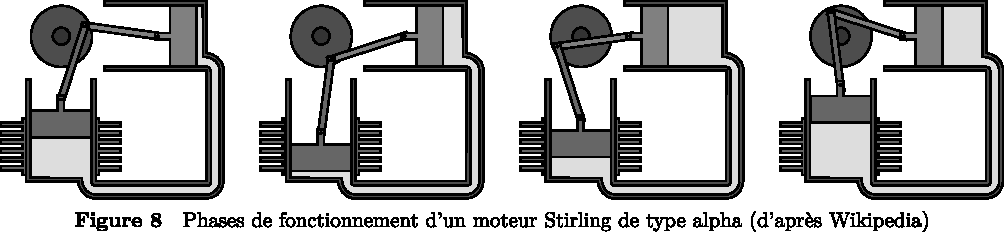
\includegraphics[scale=1]{figures/pb-stirling-fig8.pdf}

\end{center}

Le mouvement du gaz peut être décrit par 4 phases plus ou moins
distinctes (figure 8) :

\begin{itemize}
	\item
	      une phase de compression, pendant laquelle le volume de la chambre
	      chaude est minimal, le fluide, entièrement situé dans la zone froide,
	      est comprimé par le piston de travail dans sa course vers le bas ;
	\item
	      une fois le piston de travail au point mort bas, le déplaceur est
	      ramené à gauche, ce qui a pour effet de transvaser le fluide comprimé,
	      qui passe de la zone froide vers la zone chaude et reçoit un transfert
	      thermique de la source externe ;
	\item
	      une phase de détente, pendant laquelle le fluide se détend dans le
	      volume d'expansion où il continue d'être chauffé. Cette détente a pour
	      effet de repousser le déplaceur et le piston de travail ;
	\item
	      une fois que le piston de travail a atteint le point mort haut, le
	      déplaceur est ramené à droite, ce qui a pour effet de transvaser le
	      fluide de la zone chaude (volume d'expansion) vers la zone froide
	      (volume de compression). Au cours de ce transfert, le fluide cède de
	      la chaleur au refroidisseur.
\end{itemize}

Un cycle réel d'un moteur de Stirling est représenté dans le diagramme
\((p,V)\), \textbf{sur le document réponse à rendre avec la copie.}

\begin{enumerate}
	\item
	      Justifier que ce cycle est celui d'un moteur. Estimer la valeur du
	      travail fourni par le moteur pendant un cycle.
\end{enumerate}

\subsection{Modélisation du cycle}

On étudie le cycle de Stirling idéal. Au cours de celui-ci, \(n\) moles
de gaz parfait de coefficient adiabatique \(\gamma\) subissent les
transformations suivantes :

\begin{itemize}
	\item
	      une compression \((1 \to 2)\) isotherme réversible à la température
	      \(T_1\),
	\item
	      un échauffement \((2 \to 3)\) isochore jusqu'à l'état 3 de température
	      \(T_3\),
	\item
	      une détente \((3 \to 4)\) isotherme réversible à la température
	      \(T_3\),
	\item
	      un refroidissement \((4 \to 1)\) isochore jusqu'à l'état 1.
\end{itemize}

Il n'y a pas d'autre travail que celui des forces de pression.

\begin{enumerate}
	\setcounter{enumi}{1}
	\item
	      Représenter sur la figure du document réponse, à rendre avec la copie,
	      l'allure du diagramme correspondant au cycle idéal.
\end{enumerate}

On note \(r = \frac{V_1}{V_2}\) le rapport de compression entre les
volumes fixés par construction. On rappelle que la capacité thermique à
volume constant d'un gaz de \(n\) moles de gaz parfait vaut
\(C_V=\frac{nR}{\gamma -1}\) où \(R\) est la constante des gaz parfaits.

\begin{enumerate}
	\setcounter{enumi}{2}
	\item
	      Exprimer \(W_{12}\) , le travail reçu par le fluide au cours de la
	      compression, en fonction de \(n, R, T_1\) et \(r\). En déduire le
	      transfert thermique \(Q_{12}\) reçu par le fluide au cours de cette
	      compression en fonction de \(n, R, T_1\) et \(r\). Préciser les signes
	      de \(W_{12}\) et de \(Q_{12}\) .
	\item
	      Exprimer \(Q_{23}\), le transfert thermique reçu par le fluide au
	      cours de l'échauffement isochore, en fonction de \(n, R, T_1, T_3\) et
	      \(\gamma\). Préciser son signe.
	\item
	      Exprimer \(W_{34}\) , le travail reçu par le fluide au cours de la
	      détente, en fonction de \(n, R, T_3\) et \(r\). En déduire le
	      transfert thermique \(Q_{34}\) reçu par le fluide au cours de cette
	      détente en fonction de \(n, R, T_3\) et \(r\). Préciser les signes de
	      \(W_{34}\) et \(Q_{34}\).
	\item
	      Exprimer le transfert thermique \(Q_{41}\) reçu par le fluide au cours
	      du refroidissement en fonction de \(n, R, T_1 , T_3\) et \(\gamma\).
	      Préciser son signe.
\end{enumerate}

\subsection{Rendement du moteur}

\begin{enumerate}
	\setcounter{enumi}{6}
	\item
	      Définir puis exprimer le rendement idéal du moteur en fonction de
	      \(T_1 , T_3 , r\) et \(\gamma\).
	\item
	      Définir et exprimer le rendement de Carnot en fonction de \(T_1\) et
	      \(T_3\).
\end{enumerate}

Dans beaucoup de situations, le moteur de Stirling contient un
régénérateur. Dans ce cas, la chaleur perdue par le gaz lors du
refroidissement isochore \((4 \to 1)\) est récupérée par le gaz lors du
chauffage isochore \((2 \to 3)\). Si le régénérateur est idéal, cette
récupération est totale.

\begin{enumerate}
	\setcounter{enumi}{8}
	\item
	      Que devient le rendement du cycle idéal dans ce cas ?
\end{enumerate}

On considère 2 moteurs de Stirling combinés dont l'efficacité est
environ 50 \% de l'efficacité de Carnot, alimenté par une puissance
électrique d'environ 180 W.

\begin{enumerate}
	\setcounter{enumi}{9}
	\item
	      En prenant une température chaude de 640 °C et une température froide
	      de 60 °C et en supposant la conversion du travail mécanique en travail
	      électrique parfaite, estimer numériquement la puissance thermique
	      fournie par la source chaude aux deux moteurs de Stirling combinés.
\end{enumerate}

\section{Étude thermodynamique d'une chambre froide}

Le stockage des récoltes s'effectue dans une chambre froide. On se
propose dans cette partie d'étudier cette machine thermique. Le fluide
réfrigérant étudié est du R134a. Pour les futures constructions, le
fluide sera du R1234ze pour sa moindre contribution à l'effet de serre.

\subsection{Généralités}

Le fluide réfrigérant décrit le cycle thermodynamique présenté figure 8.
On modélise la machine frigorifique par une machine ditherme schématisée
en figure 9.

On utilise les notations suivantes :

\begin{itemize}
	\item
	      \(Q_c\) : transfert thermique algébriquement reçu par le fluide au
	      cours d'un cycle de la part de la source chaude à la température
	      \(T_c\);
	\item
	      \(Q_f\) : transfert thermique algébriquement reçu par le fluide au
	      cours d'un cycle de la part de la source froide à la température
	      \(T_f\);
	\item
	      \(W\) : travail algébriquement reçu par le fluide au cours d'un cycle
	      de la part de l'extérieur.
\end{itemize}

\begin{center}

	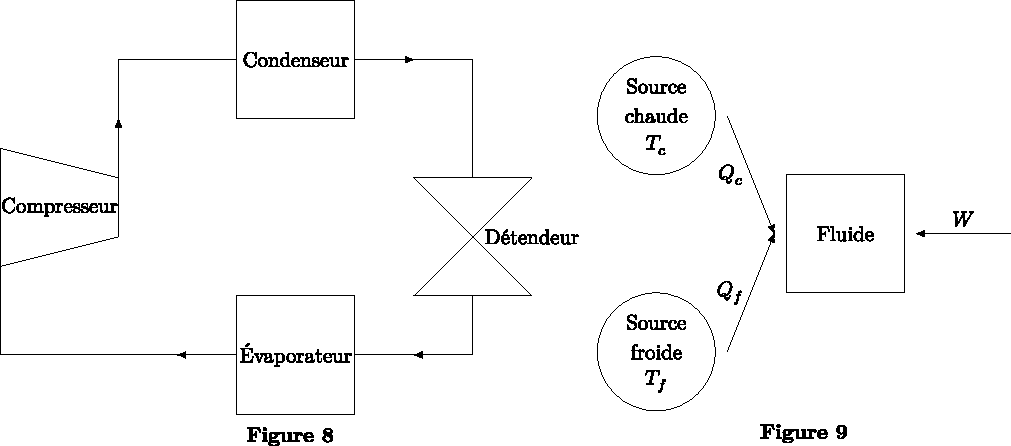
\includegraphics[scale=1]{figures/pb-chambre-fig89.pdf}

\end{center}

\begin{enumerate}
	\item
	      Au niveau de quel organe de la machine thermique se trouve la chambre
	      froide ? Justifier votre réponse.
	\item
	      Préciser en justifiant les signes de \(Q_c,Q_f\) et \(W\).
	\item
	      Définir l'efficacité \(e\) (également appelé COefficient de
	      Performance COP) de la machine frigorifique.
	\item
	      Établir l'expression de l'efficacité de Carnot \(e_c\), en fonction de
	      \(T_c\) et \(T_f\). Que peut-on dire l'efficacité réelle \(e\) par
	      rapport à l'efficacité de Carnot \(e_c\)?
	\item
	      Calculer numériquement \(e_c\) avec \(T_c = 45\ ^\circ\mathrm{C}\) et
	      \(T_f = 3\ ^\circ\mathrm{C}\). Interpréter le résultat obtenu.
\end{enumerate}

\subsection{Description du cycle}

Le cycle comprend les successions de transformations suivantes :

\begin{itemize}
	\item
	      \(1 \to 2\) : compression adiabatique réversible en phase gazeuse dans
	      le compresseur ;
	\item
	      \(2 \to 3\) : refroidissement isobare de la vapeur ;
	\item
	      \(3 \to 4\) : compression totale et isobare ;
	\item
	      \(4 \to 5\) : sous-refroidissement isobare ;
	\item
	      \(5 \to 6\) : détente isenthalpique ;
	\item
	      \(6 \to 7\) : chauffage isobare ;
	\item
	      \(7 \to 1\) : surchauffe de la vapeur.
\end{itemize}

Le tableau 2 donne le relevé thermodynamique du fluide aux différents
points de ce cycle.

\begin{center}

	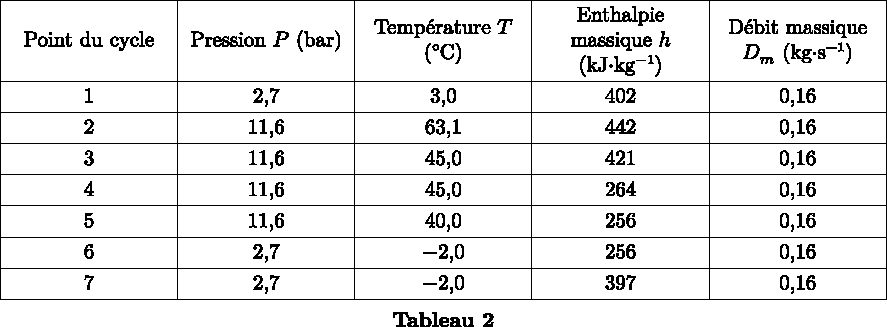
\includegraphics[scale=1]{figures/pb-chambre-tab2.pdf}

\end{center}

\begin{enumerate}
	\setcounter{enumi}{5}
	\item
	      Représenter le cycle thermodynamique sur le diagramme des frigoristes
	      \((p,h)\) du document réponse.
	\item
	      Qualifier l'état du fluide aux points 3 et 4.
	\item
	      Lire graphiquement le titre en vapeur \(x_v\) du point 6.
	\item
	      Rappeler l'expression du premier principe de la thermodynamique pour
	      un fluide en écoulement stationnaire, dans lequel on néglige les
	      variations d'énergie cinétique massique \(\Delta e_c\) et d'énergie
	      potentielle de pesanteur massique \(\Delta e_p\) devant la variation
	      d'enthalpie massique \(\Delta h\).
	\item
	      Exprimer puis calculer numériquement le transfert thermique massique
	      \(q_f\) reçu par le fluide dans l'évaporateur.
	\item
	      Exprimer puis calculer numériquement le transfert thermique massique
	      \(q_c\) reçu par le fluide dans le condenseur.
	\item
	      Exprimer puis calculer numériquement le travail indiqué \(w_i\) reçu
	      par le fluide de la part du compresseur.
	\item
	      En déduire l'efficacité réelle \(e\) de la machine frigorifique.
	\item
	      Exprimer puis calculer numériquement la puissance thermique extraite
	      de la chambre froide \(P_{th,f}\).
\end{enumerate}

\newpage

\section{Étude de deux gaz parfaits dans un cylindre}

Deux gaz, supposés parfaits, sont enfermés dans deux compartiments (1)
et (2) séparés par un piston mobile athermane (on dit aussi calorifugé)
qui coulisse sans frottement. Le compartiment (1) est entièrement
calorifugé tandis que le compartiment (2) peut échanger de l'énergie par
chaleur (transfert thermique) avec le milieu extérieur, assimilé à un
thermostat de température \(T_0\) , à travers une paroi diathermane fixe
(non calorifugée).

Les deux compartiments contiennent chacun \(n\) moles de gaz et sont,
dans l'état initial, à la température \(T\) . Le volume total des deux
compartiments est \(V_t = 2V_0\) , où \(V_0\) désigne les volumes,
initialement égaux, de chacun des deux compartiments.

\begin{center}

	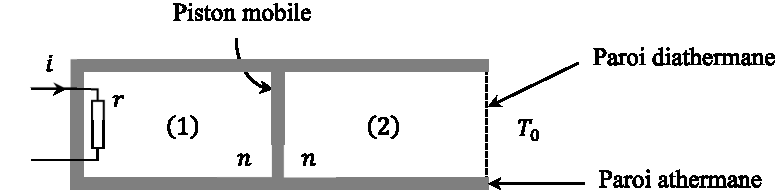
\includegraphics[scale=1]{figures/pb-2gaz.pdf}

\end{center}

À un instant pris comme origine temporelle, le compartiment (1) reçoit
de la chaleur par l'intermédiaire d'un résistor (résistance \(r\))
alimentée pendant une durée \(\tau\), par un générateur qui délivre un
courant d'intensité \(i\) constante.

L'état final est l'état d'équilibre thermodynamique du système qui
succède à ce chauffage. On le caractérise par les variables d'état
\(P_k , V_k\) et \(T_k\) qui représentent les pressions, volumes et
températures des compartiments \((k)\) où \(k = 1\) ou \(2\).

On note \(R\) la constante des gaz parfaits et
\(\gamma = \frac{C_{pm}}{C_{vm}}\) le rapport de la capacité thermique
molaire à pression constante sur la capacité thermique molaire à volume
constant, identique pour les gaz des deux compartiments.

\begin{center}

	\textbf{Indiquer la (ou les) bonne(s) réponse(s) en justifiant tout
		votre raisonnement.}

\end{center}

\begin{enumerate}
	\item
	      Exprimer \(V_1\) et \(V_2\)
	      \[ A) \ V_1 = \frac{T_1}{T_0 + T_1}V_0 \qquad\qquad B) \ V_1 = \frac{T_1}{T_0 + T_1}V_t \ \qquad\qquad C) \ V_2 = \frac{T_0}{T_0 + T_1}V_0 \qquad\qquad D) \ V_2 = \frac{T_0}{T_0 + T_1}V_t\]
	\item
	      Que peut-on affirmer ?
	      \[ A) \ P_1 = P_2 \qquad\qquad B) \ P_1 = \frac{nR(T_0 + T_1)}{V_t} \ \qquad\qquad C) \ P_1 = \frac{nR(T_0 + T_1)}{V_0} \qquad\qquad D) \ P_1 \neq P_2\]
	\item
	      Déterminer la variation d'énergie interne \(\Delta U\) entre l'état
	      initial et l'état final du système constitué par les deux gaz (on
	      indique que \(\Delta U\) est la somme des variations des énergies
	      internes des deux gaz, entre l'état initial et final) :
	      \[ A) \ \Delta U = 0 \qquad\qquad B) \ \Delta U = \frac{nR}{\gamma -1}(T_1 - T_0) \ \qquad\qquad C) \ \Delta U = \frac{nR\gamma}{\gamma -1}(T_1 - T_0) \qquad\qquad D) \ \Delta U = nR(T_1 - T_0)\]
\end{enumerate}

\emph{On supposera dans toute la suite que la transformation du
	compartiment (2) est réversible.}

\begin{enumerate}
	\setcounter{enumi}{3}
	\item
	      On note \(W\) et \(Q\) le travail et la chaleur (transfert thermique)
	      algébriquement reçus par le gaz du compartiment (2) entre l'état
	      initial et l'état final. Que peut-on affirmer ?
	      \[ A) \ W_2 = nRT_0\ln\left(\frac{T_0 + T_1}{2T_0}\right) \qquad\qquad B) \ W_2 = 0 \ \qquad\qquad C) \ Q_2 = 0 \qquad\qquad D) \ Q_2 = -W_2\]
	\item
	      On note \(Q\) la chaleur (transfert thermique) algébriquement reçu par
	      le gaz du compartiment (1) entre l'état initial et l'état final. Que
	      peut-on affirmer ?
	      \[ A) \ Q_1 = \Delta U \qquad\qquad B) \ Q_1 = \Delta U + W_1 \ \qquad\qquad C) \ Q_1 = W_2 \qquad\qquad D) \ Q_1 = ri^2\tau\]
\end{enumerate}

On note \(S_2^{(r)}\) l'entropie algébriquement reçue et \(S_2^{(c)}\)
l'entropie algébriquement créée, entre l'état initial et l'état final,
pour le gaz situé dans le compartiment (2). On indique que sa variation
d'entropie \(\Delta S_2\) entre l'état initial et l'état final s'écrit
\(\Delta S_2 = nR \ln\left(\frac{V_2}{V_0}\right)\).

\begin{enumerate}
	\setcounter{enumi}{5}
	\item
	      Exprimer \(S_2^{(r)}\) et \(S_2^{(c)}\)
	      \[ A) \ S_2^{(r)} = nR\ln\left(\frac{2T_0}{T_0 + T_1}\right) \qquad\qquad B) \ S_2^{(r)} = 0 \ \qquad\qquad C) \ S_2^{(c)} = nR\ln\left(\frac{2T_0}{T_0 + T_1}\right) \qquad\qquad D) \ S_2^{(c)} = 0\]
\end{enumerate}

\section{Cycle de Carnot}

\subsection{Chaleur perdue et machine thermique}

Les enjeux de la transition énergétique amènent des réflexions sur
l'efficacité des systèmes de production et de conversion de l'énergie,
ainsi que sur la récupération d'énergie. Optimiser les systèmes de
production d'énergie et récupérer le plus d'énergie possible lors d'une
conversion d'énergie deviennent des sujets majeurs dans le cadre d'une
politique d'économie d'énergie.

Lors du fonctionnement d'un procédé industriel, l'énergie thermique
produite grâce à l'énergie apportée n'est pas utilisée en totalité. Une
partie de la chaleur est inévitablement rejetée et non récupérée. En
raison de ce caractère inéluctable, on parle de \emph{chaleur fatale}.
Cette quantité d'énergie perdue constitue un gisement potentiel à
récupérer.

Cependant, cette appellation est en partie erronée car la chaleur fatale
peut être en partie récupérée. L'ADEME (Agence De l'Environnement et de
la Maîtrise de l'Energie) classe le gisement de chaleur fatale
disponible par écart de température par rapport à la température
ambiante (source froide).

Le tableau ci-dessous donne les gisements de chaleur fatale (Énergie
thermique) disponible par an et classés par écart de température avec la
température ambiante, ici prise à $\SI{27}{\degreeCelsius}$.

\begin{center}
	\begin{tabular}{cc}
		\toprule
		Écart de température     & Gisement
		\\
		\midrule
		\(30\ ^\circ\mathrm{C}\) & \(20\ \mathrm{TWh}\)
		\\
		\(75\ ^\circ\mathrm{C}\) & \(20\ \mathrm{TWh}\)
		\\
		\bottomrule
	\end{tabular}
\end{center}

\begin{enumerate}
	\item
	      Rappeler l'expression du premier principe et du deuxième principe de
	      la thermodynamique. Que deviennent ces expressions sur un cycle
	      thermodynamique ?
\end{enumerate}

On considère un système thermodynamique quelconque, noté
\(\mathcal{S}\), en contact avec deux thermostats aux températures
\(T_\mathrm{ch}\) et \(T_\mathrm{fr}\) avec
\(T_\mathrm{ch} > T_\mathrm{fr}\). On note \(Q_C\) la chaleur échangée
entre le système \(\mathcal{S}\) et la source \(T_\mathrm{ch}\) , et
\(Q_F\) la chaleur échangée entre le système \(\mathcal{S}\) et la
source \(T_\mathrm{fr}\).

\begin{enumerate}
	\setcounter{enumi}{1}
	\item
	      Rappeler le nom et la définition des transformations associées à un
	      cycle de Carnot subi par le système \(\mathcal{S}\), en contact avec
	      les deux thermostats précédents. On représentera les étapes du cycle
	      dans le plan \((T,S)\) en faisant apparaitre clairement les
	      températures des thermostats.
	\item
	      Dans le cas d'un système subissant un cycle de Carnot, réaliser un
	      bilan d'énergie et un bilan d'entropie, et en déduire l'expression du
	      rendement \(\eta\) en fonctionnement moteur en fonction de
	      \(T_\mathrm{ch}\) et \(T_\mathrm{fr}\).
	\item
	      À partir des données du tableau précèdent, justifier pourquoi l'ADEME
	      classe les gisements par écart de température par rapport à la
	      température de la source froide et en déduire en Wh l'énergie que l'on
	      pourrait récupérer par an et par gisement.
\end{enumerate}

\subsection{Machine de Carnot opérée avec un gaz parfait}

Considérons le système \(\mathcal{S}\) précédent comme étant un gaz
parfait et subissant un cycle de Carnot entre \(T_\mathrm{ch}\) et
\(T_\mathrm{fr}\) , respectivement à 57°C et 27°C. À chaque état du
cycle, le volume, la pression et la température du système
\(\mathcal{S}\) sont indicés successivement par 1, 2, 3 et 4.

L'état 1 du cycle correspond au moment juste avant la phase de
compression adiabatique. Dans cet état, le système est dans un volume de
1 cm × 1cm × 1mm (noté \(V_1\)), la pression est de 1 bar (notée
\(P_1\)) et sa température est \(T_1 = T_\mathrm{fr}\) . On notera que
sur la phase d'échange de chaleur avec la source chaude, la variation de
pression est de 0,4 bar.

On note \(c_p\) et \(c_v\) les capacités thermiques massiques du système
à pression constante et à volume constant, respectivement, en
\(\mathrm{J.K^{-1}.kg^{-1}}\). On rappelle que ces capacités thermiques
obéissent à la relation de Mayer : \(c_p - c_v = \frac{R}{M}\), où \(R\)
est la constante universelle des gaz parfaits, et \(M\) la masse
molaire. On considère dans la suite que le système \(\mathcal{S}\) est
constitué d'air, assimilé à un gaz parfait diatomique, tel que l'indice
adiabatique \(\gamma = \frac{c_p}{c_v}\) vaut 7/5.

\begin{enumerate}
	\setcounter{enumi}{4}
	\item
	      Caractériser qualitativement la variation de pression du système
	      \(\mathcal{S}\) le long du cycle, en détaillant les transformations
	      entre chaque état thermodynamique: \(1 \to 2, 2 \to 3, 3 \to 4\) et
	      \(4 \to 1\).
	\item
	      Donner l'expression de la dérivée \(\dv{P}{V}\) pour chaque
	      transformation en fonction de \(\gamma, P\) et \(V\) et représenter
	      les étapes du cycle dans le plan \((P,V)\).
\end{enumerate}

Pour un gaz parfait, la variation infinitésimale d'entropie
\(\mathrm{d} S\) s'exprime en fonctions des variations infinitésimales
de température \(\mathrm{d} T\) et de pression \(\mathrm{d} P\):
\[\mathrm{d}S = \frac{m c_p}{T} \mathrm{d}T - \frac{nR}{P}\mathrm{d}P \]
avec \(n\) la quantité de matière et \(m\) la masse du gaz.

\begin{enumerate}
	\setcounter{enumi}{6}
	\item
	      Exprimer \(\mathrm{d}S\) en fonction en fonction de
	      \(P_1 , V_1, T_1\), et des capacités thermiques massiques. On ne fera
	      pas intervenir dans le résultat \(n\) et \(m\).
	\item
	      Calculer les valeurs numériques des pressions \(P_1,P_2,P_3\) et
	      \(P_4\).
	\item
	      Exprimer les chaleurs échangées \(Q_\mathrm{ch}\) en fonction de
	      \(P_1 , V_1, T_1, T_\mathrm{ch}, P_2/P_3\) et \(Q_\mathrm{fr}\) en
	      fonction de \(P_1 , V_1 , T_1, T_\mathrm{fr} , P_4/P_1\). Évaluer
	      numériquement \(Q_\mathrm{ch}\) et \(Q_\mathrm{fr}\).
	\item
	      En déduire l'expression et la valeur numérique du travail mécanique
	      récupéré pour un cycle moteur. Le résultat paraît-il cohérent avec la
	      valeur obtenue si on utilise l'expression du rendement de Carnot ?
	\item
	      Les machines thermiques de récupération de chaleur fatale fonctionnent
	      en réalité avec deux transformations isobares pour des raisons
	      techniques. Expliquer pourquoi un fluide subissant une transition de
	      phase (un changement d'état ici) permet d'améliorer l'efficacité de la
	      machine thermique.
\end{enumerate}

%% Document réponse à rendre (doit être en page impaire!)
\newpage

\begin{tcolorbox}
	\centering\huge{\textbf{Document réponse \\\emph{A rendre avec la copie}}}
\end{tcolorbox}

\textbf{Nom: \hspace{7cm} Prénom:}\\

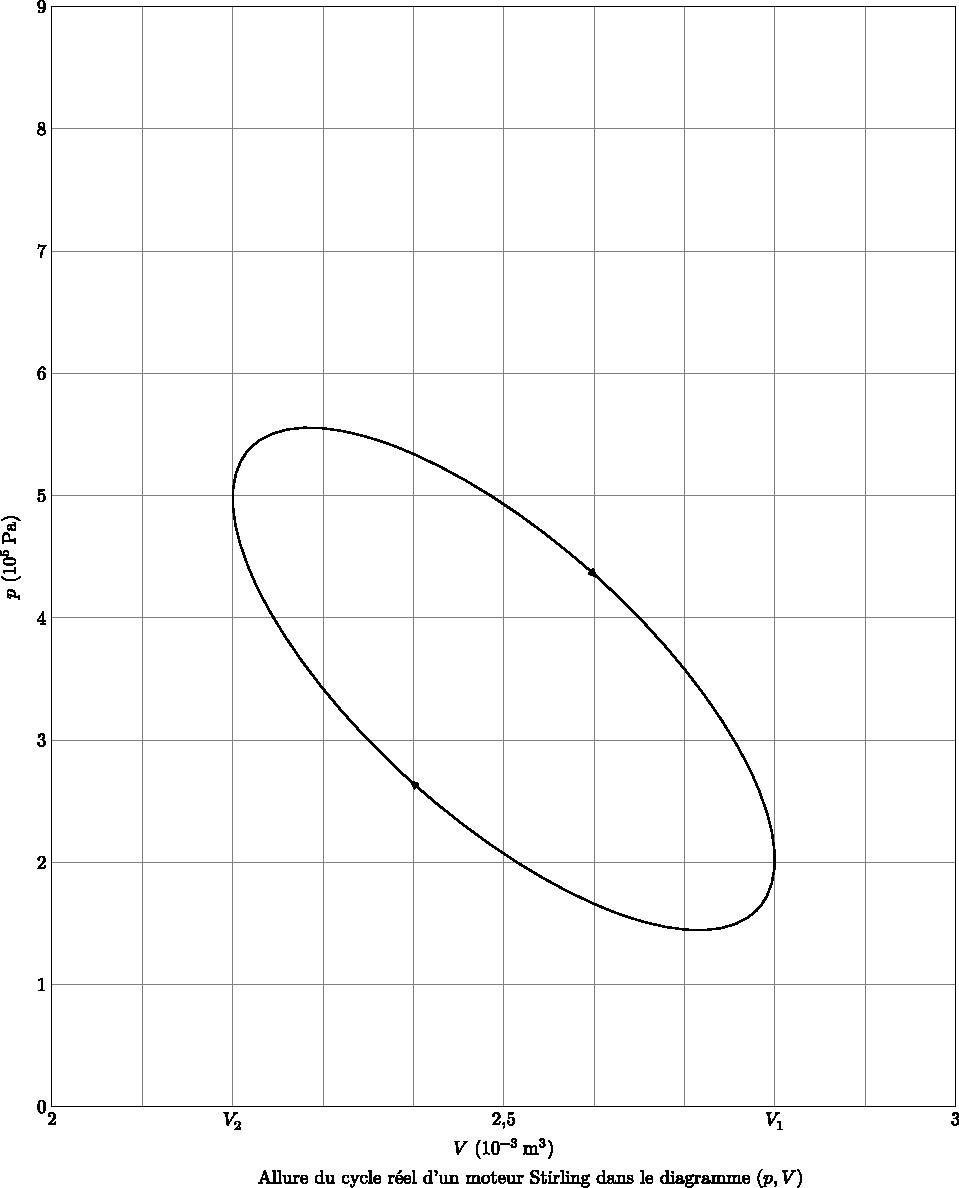
\includegraphics[scale=1]{figures/pb-stirling-cycle.pdf}

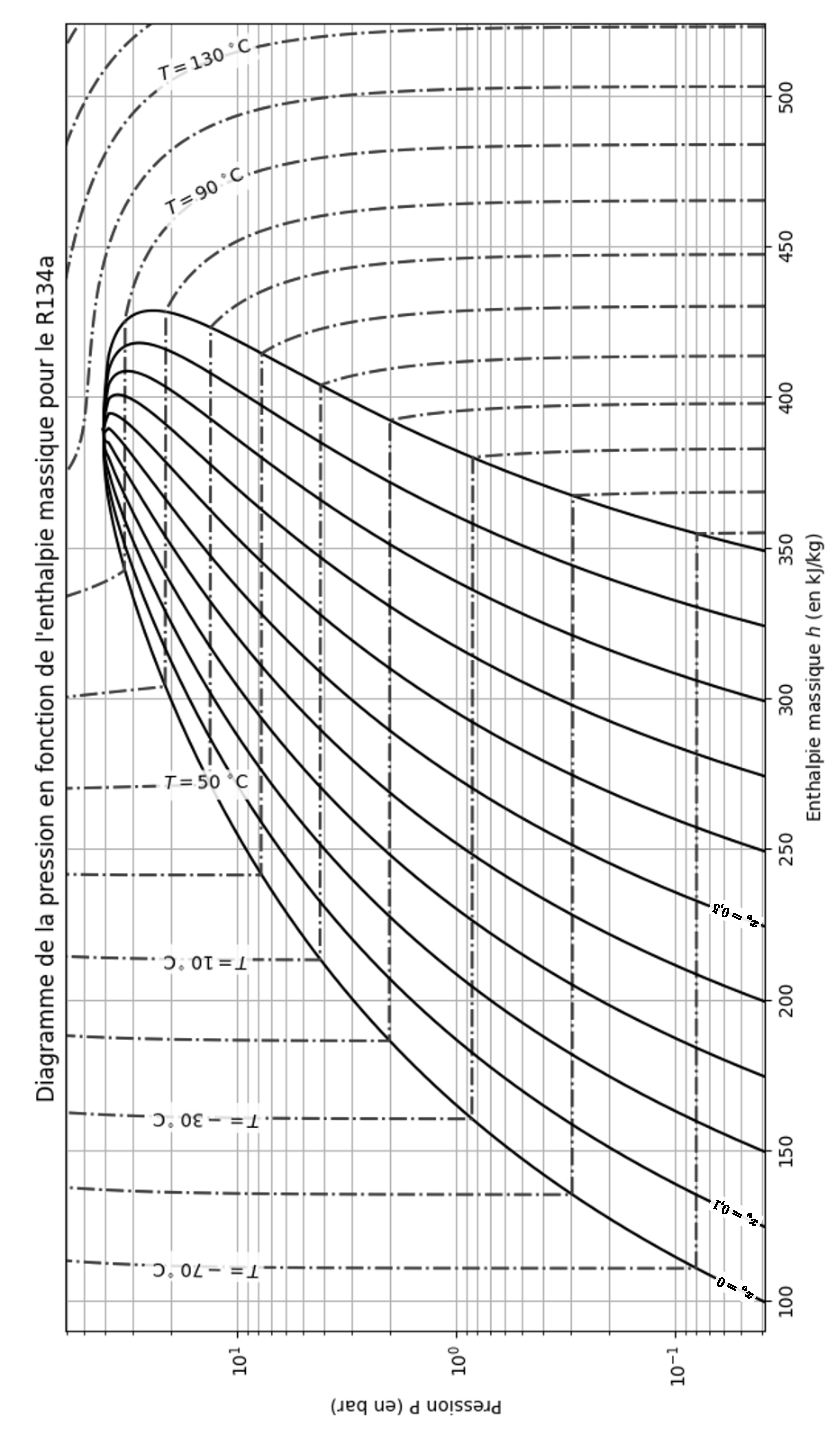
\includegraphics[scale=1]{figures/pb-chambre-ph.pdf}


\end{document}
